
\section{Introduction}
\label{sec:intro}
In the recent years, our information society has reached the stage where it produces billions of data records, amounting to multiple quintillion of bytes\furl{https://www.domo.com/learn/data-never-sleeps-5}, on a daily basis.
Extraction, cleansing, enrichment and refinement of information are key to fuel value-adding processes, such as analytics as a premise for decision making.
% add value or something
Devising appropriate (ideally uniform) representations and facilitating efficient querying of data, metadata and provenance arising from such phases constantly poses challenges, especially when data volumes are vast. %For a better representation and capable of extracting desired information there is an effort of better representing such a large amount of data (e.g. metadata).
%The efforts have been made constantly.
The most prominent and promising effort is the W3C consortium with encouraging Resource Description Framework (RDF)\furl{https://www.w3.org/TR/rdf11-primer/} as a common data representation and vocabularies (e.g. RDFS, OWL) as a way to include meta-information about the data.
These data and meta-data can be further processed and analyzed using the de-facto query language for RDF data, SPARQL\furl{https://www.w3.org/TR/sparql11-overview/}.

SPARQL serves as a standard query language for manipulating and retrieving RDF data.
Querying RDF data becomes challenging when the size of the data increases. 
Recently, many distributed RDF systems capable of evaluating SPARQL queries have been proposed and developed (\cite{Schatzle:2016:SRQ:2977797.2977806}, \cite{sparqlgx-iswc-2016}).
Nevertheless, these engines lack one important information derived from the knowledge, \emph{RDF terms}.
RDF terms includes information about a statement such as \emph{language}, \emph{typed literals} and \emph{blank nodes} which are omitted from most of the engines.

To cover this spectrum requires a specialized system which is capable of constructing an efficient SPARQL query engine. 
Doing so comes with several challenges.
First and foremost, recently the RDF data is increasing drastically.
Just as a record, today we count more than 10,0000 datasets\furl{http://lodstats.aksw.org/} available online represented using the Semantic Web standards.
This number is increasing daily including many other (e.g Ethereum\furl{https://goo.gl/mJTkPp} dataset) datasets available at the organization premises.
In addition, being able to query this large amount of data in an efficient and faster way is a requirement from most of the SPARQL evaluators.

To overcome these challenges, in this paper, we propose \emph{Sparklify}\furl{https://github.com/SANSA-Stack/SANSA-Query/tree/develop/sansa-query-spark/src/main/scala/net/sansa_stack/query/spark/sparqlify}: a scalable software component for efficient evaluation of SPARQL queries over distributed RDF datasets. The conceptual foundation is the application of \emph{ontology-based data access} (OBDA) tooling, specifically SPARQL-to-SQL rewriting, for translating SPARQL queries into Spark executable code. We demonstrate our approach using Sparqlify, which has been used in the LinkedGeoData\furl{http://linkedgeodata.org} community project to serve more than 30 billion triples on-the-fly from a relational OpenStreetMap database.
Our contributions are:
\begin{itemize}
 \item We present a novel approach for vertical partitioning including RDF terms using the distributed computing framework, Apache Spark.
 \item We developed a scalable query engine using Sparqlify -- a SPARQL-to-SQL rewriter on top of Apache Spark (under the \textit{Apache Licence 2.0}).
 \item We evaluate our approach with state-of-the-art engines and demonstrate it empirically.
 \item We integrated the approach into the SANSA~\cite{lehmann-2017-sansa-iswc}\furl{http://sansa-stack.net/} larger framework.
 Sparklify serves as a default query engine in SANSA.
 SANSA is an active project and maintained, including issue tracker, mailing list, changelogs, website, etc.
\end{itemize}

The paper is structured as follows:
Our approach for data modeling and query translation using a distributed framework is detailed in \autoref{sec:approach} and evaluated in \autoref{sec:evaluation}.
Related work on the SPARQL query engines is discussed in \autoref{sec:related_work}.
Finally, we conclude and suggest planned extensions of our approach in \autoref{sec:conclusion}.

\section{Preliminaries}
\label{sec:preliminaries}
In this section, we first introduce the basic notions used in throughout the paper.

%\begin{definition}[RDF Graph]
%\label{def:rdf_graph}
%Let $\mathcal{U}$, be a set of URIs, $\mathcal{B}$ set of blank nodes and $\mathcal{L}$ set of literals, an RDF Graph ($\mathcal{G}$) is defined as a set of triples in the form of ${(s, p, o) \in (\mathcal{U} \cup \mathcal{B}) \times \mathcal{U} \times (U \cup B \cup L)}$, where the subject $s \in (U \cup B)$ is a resource, the predicate $p \in U$ is a property, and the object $o \in (\mathcal{U} \cup \mathcal{B} \cup \mathcal{L})$ is either another resource ($\mathcal{U} \cup \mathcal{B}$) or a literal ($\mathcal{L}$). 
%\end{definition}

%\begin{definition}[SPARQL]
%\label{def:sparql}
%A SPARQL query $Q$ is a tuple of $(query-type,$ $pattern~P, modifiers)$, where, $query-type$ in our case is a \emph{SELECT} queries.
%A \emph{pattern} $P$ contains patterns which are matched against RDF data $\mathcal{G}$.
%The \emph{modifiers} are aggregations, grouping, sorting, distinct, and a slice of the result set mapped from the pattern $P$.
%\end{definition}

\subsection{Sparqlify}
Sparqlify\furl{https://github.com/SmartDataAnalytics/Sparqlify} is a SPARQL-to-SQL rewriter that enables answering SPARQL queries on relational databases via a set of view definitions. R2RML\furl{https://www.w3.org/TR/r2rml/} and the more intuitive \textit{Sparqlification Mapping Language(SML)}\furl{http://sml.aksw.org/}~\cite{sml} are supported. In general, the rewriter compiles every SPARQL query into two related artifacts: A SQL query and set of SPARQL result variable definitions by means of expressions over the SQL query's result set.
Sparqlify first converts the query into an algebra expression. Subsequently, algebraic optimizations and normalizations are applied, such as filter placement and constant folding.
Given a query pattern, the view selection component identifies for every triple pattern the set of candidate view definitions together with the renaming of their variables to those of the requesting pattern. This is the base for obtaining the final algebra expression. In general, this involves a cartesian product between triple patterns and views definitions, which leads to a union of joins between the candidate views. Pruning is performed based on RDF term types and IRI prefixes: Choosing a view that binds variables to certain term types or prefixes will constrain subsequent loops only to those candidates with compatible bindings for these variables.
%These constraints propagate.
%It comes with a powerful optimization which analyze these algebra expression for improving the efficiency.
Finally, this algebra expression are transformed into an SQL algebra expression using the general relational algebra for RDB-to-RDF mappings.
The SQL query, which has been obtained, is used further (e.g. in our case for executing it over Spark SQL engine).

\subsection{Apache Spark}
Apache Spark is a fast and generic-purpose cluster computing engine which is built over Hadoop ecosystem.
Its core data structure are Resilient Distributed Dataset (RDD)~\cite{zaharia2012resilient} which are a fault-tolerant and immutable collections of records that can be operated in a parallel setting.
Spark also provides high-level APIs, and tools, including Spark SQL~\cite{Armbrust2015SSR} for SQL and structured data processing which allows querying structured data inside Spark programs.
In this work, we make use of the above libraries from the Apache Spark stack.


\begin{figure*}[t]
\centering
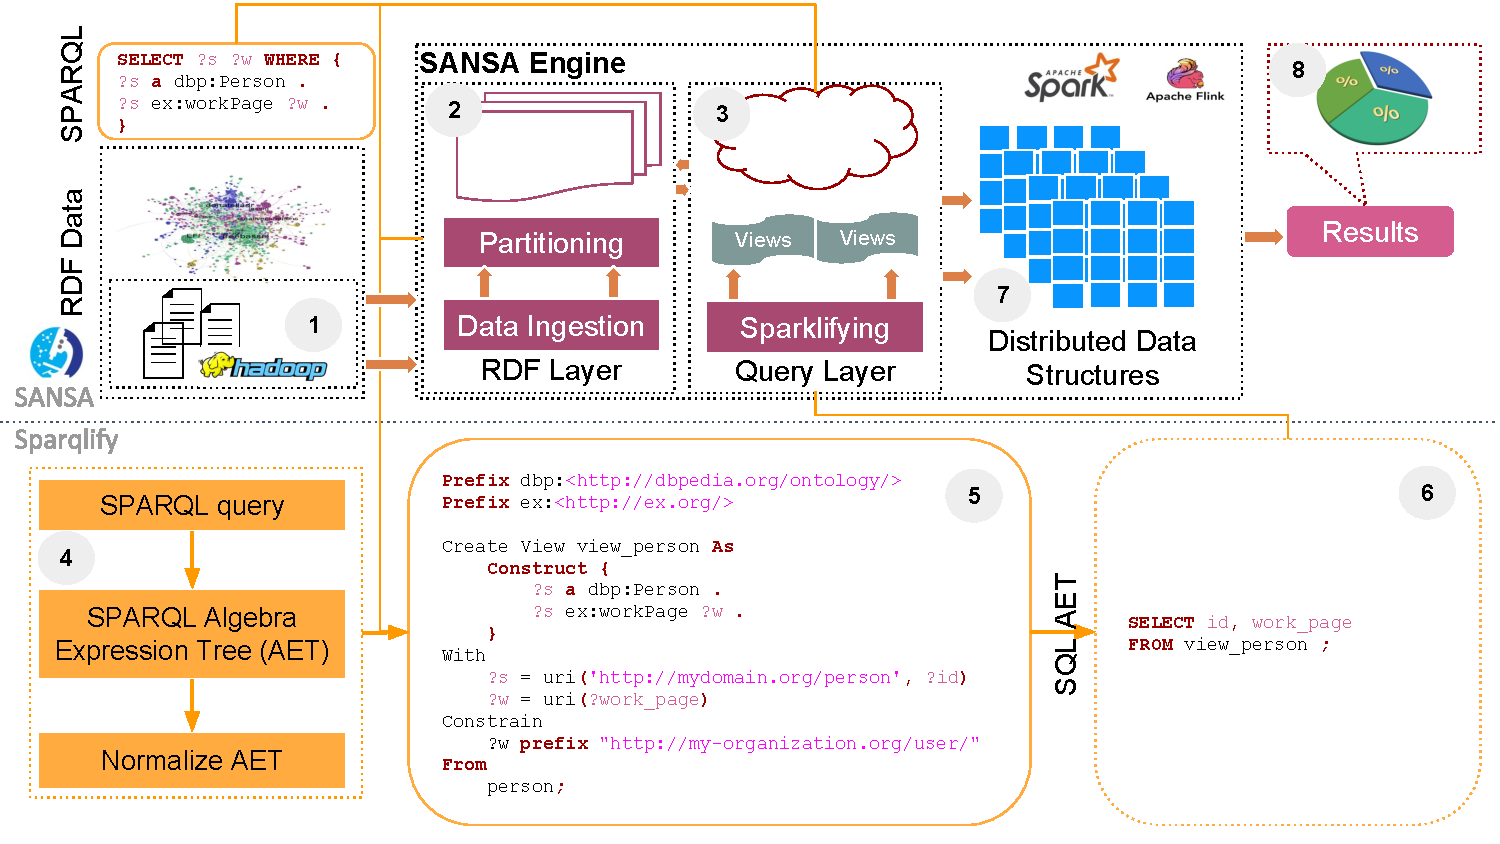
\includegraphics[width=1.0\textwidth]{images/sparklify-architecture.pdf}
\caption{Sparklify Architecture Overview.}
% source : https://docs.google.com/presentation/d/16XlT4u3bFn8XdP_eoLJOAu5WPl_q_9zIjAZbllfEEic/edit?usp=sharing 
\label{fig:architecture}
% source : 
\end{figure*}

\section{Sparklify}
\label{sec:approach}

In this section, we present the overall architecture of our proposed approach, the SPARQL-to-SQL rewriter, and mapping to Spark Scala-compliant code.

\subsection{System Architecture}
The overall system architecture is shown in \autoref{fig:architecture}.
It consists of four main components: Data Model, Mappings, Query Translator and Query Evaluator.
In the following, each component is discussed in details.

\subsubsection{Data Model}
SANSA~\cite{lehmann-2017-sansa-iswc} comes with different data structures and different partitioning strategies.
We model and store RDF graph following the concept of RDDs -- a basic building blocks of the Spark Framework.
RDDs are in-memory collections of records which are capable of operating in parallel overall larger cluster.
Sparklify makes use of SANSA bottom layer which corresponds with the extended vertical partitioning (VP) including RDF terms.
This partition model is the most convenient storage model for fast processing of RDF datasets on top of HDFS.
\paragraph{Data Ingestion (step 1)} RDF data first needs to be loaded into a large-scale storage that Spark can efficiently read from.
We use Hadoop Distributed File-System (HDFS)\furl{https://hadoop.apache.org/docs/r1.2.1/hdfs_design.html}.
Spark employ different data locality scheme in order to accomplish computations nearest to the desired data in HDFS, as a result avoiding i/o overhead. 
\paragraph{Data Partition (step 2)}
VP approach in SANSA is designed to support extensible partitioning of RDF data.
Instead of dealing with a single three-column table $(s, p, o)$, data is partitioned into multiple tables based on the used RDF predicates, RDF term types and literal datatypes.
The first column of these tables is always a string representing the subject.
The second column always represents the literal value as a Scala/Java datatype.
Tables for storing literals with language tags have an additional third string column for the language tag.
\subsubsection{Mappings/Views}
After the RDF data has been partitioned using the extensible VP (as it has been described on \textit{step 2}) the relational-to-RDF mapping is performed. 
Sparqlify supports both the W3C standard R2RML
sparqlification~\cite{sml}.

The main entities defined with SML are \textit{view definitions}.
See \textit{step 5} in the \autoref{fig:architecture} as an example.
The actual view definition is declared by the \emph{Create View} \ldots \emph{As} in the first line.
The remainder of the view contains these parts: (1) the \emph{From} directive defines the logical table based on the partitioned table (see \textit{step 2}).
(2) an RDF template is defined in the \emph{Construct} block containing, URI, blank node or literals constants (e.g. \emph{ex:worksAt}) and variables (e.g. \emph{?emp}, \emph{?institute}).
The \emph{With} block defines the variables used in the template by means of RDF term constructor expressions whose arguments refer to columns of the logical table.

\subsubsection{Query Translation}
This process generates a SQL query from the SPARQL query using the bindings determined in the mapping/view construction phases.
It walks through the SPARQL query (\textit{step 4}) using Jena ARQ\furl{https://jena.apache.org/documentation/query/} and generates the SPARQL Algebra Expression Tree (AET). Essentially, rewriting SPARQL basic graph patterns and filters over views yields AETs that are UNIONS of JOINS.
%AET are .... \fixme{Gezim: complete the sentence}
Further, these AETs are normalized and pruned in order to remove UNION members that are known to yield empty results, such as joins based on IRIs with disjoint sets of known namespaces, or joins between different RDF term types (e.g. literal and IRI).
Finally, the SQL is generated (\textit{step 6}) using the bindings corresponding to the views (\textit{step 5}).

\subsubsection{Query Evaluator}
The SQL query created as described in the previous section can now be evaluated directly into the Spark SQL engine.
The result set of this SQL query is distributed data structure of Spark (e.g. DataFrame)(\textit{step 7}) which then is mapped into a SPARQL bindings.
The result set can further used for analysis and visualization using the SANSA-Notebooks (\textit{step 8})~\cite{iermilov-2017-sansa-iswc-demo}.

\subsection{Algorithm Description}
\label{subsection:algorithm}
The algorithm described in this paper has been implemented using the Apache Spark framework (see \autoref{alg:sparklify}). 
It constructs the graph (\autoref{line:sparklify_rdf2rdd}) while reading RDF data and converts it into RDD of triples.
After, it partitions the data (\autoref{line:sparklify_partitiongraph}, for more details see \autoref{alg:partitionGraph}) using the vertical partitioning (VP) strategy.
Finally, the query evaluator is constructed (\autoref{line:sparklify_sparql}) which is described into more details in \autoref{alg:sparql} for consistency.

\begin{algorithm}[t]
\caption{Sparklify algorithm.}
\label{alg:sparklify}
\SetKwInOut{Input}{input}\SetKwInOut{Output}{output}
\Input{$q$: a SPARQL query, $input$: an RDF dataset}
\Output{$df$ list of result set}
    $\textit{graph} = spark.\textbf{rdf}(lang)(input)$ \label{line:sparklify_rdf2rdd}\\
    $\textit{graph}.persist()$\\
    $partitionGraph \leftarrow graph.\textbf{partitionGraph}()$ \label{line:sparklify_partitiongraph}\\
    $result \leftarrow partitionGraph.\textbf{sparql}(q)$ \label{line:sparklify_sparql}\\
\Return{$result$}
\end{algorithm}

\subsubsection{Partitioning the Graph}
The partitioning algorithm (see \autoref{alg:partitionGraph}) transforms the RDF graph into a convenient VP including RDF terms (\autoref{line:partitionGraph_partitioner}).
For each triple in the graph in a distributed fashion, it does the following: It gets the RDF terms about subjects and objects (\autoref{line:partitionGraph_RDFTerms}).
In case of a literal it assigns the data type for a given column while partitioning the data to: \textit{String} (\autoref{line:partitionGraph_isString}) when is plain literal, otherwise gets the data type of a given literal (e.g. \textit{Integer}, \textit{Double}) (\autoref{line:partitionGraph_LiteralDatatype}).
The remaining block is the language tag (\autoref{line:partitionGraph_languageTag}) which is required for an extra column on the partitioned table containing the language tag value.
After all this information is populated, the partitioned block is performed using the \emph{map} transformation function of Spark splitting the tables based on the above information.

\begin{algorithm}[t]
\caption{PartitionGraph algorithm.}
\label{alg:partitionGraph}
\SetKwInOut{Input}{input}\SetKwInOut{Output}{output}
\Input{$graph$: an RDD[Triple] dataset}
\Output{$views$ a mapped views}
    \ForEach{$triple \in graph$}{
        $s \leftarrow triple.getSubject; o \leftarrow triple.getObject$\\
        $subjectType \leftarrow getRDFTermType(s); objectType \leftarrow getRDFTermType(o)$ \label{line:partitionGraph_RDFTerms}\\
        $predicate \leftarrow triple.getPredicate.getURI$\\
        \eIf{o.isLiteral}{
        \eIf{isPlainLiteral(o)}{
            $datatype \leftarrow XSD.xstring.getURI$ \label{line:partitionGraph_isString}
            }{
            $datatype \leftarrow o.getLiteralDatatypeURI$ \label{line:partitionGraph_LiteralDatatype}
            }}{
        $datatype \leftarrow string.Empty$
        }
        $langTagPresent \leftarrow isPlainLiteral(o)$ \label{line:partitionGraph_languageTag} \\
        $views.add(partitioner(subjectType,predicate, objectType, datatype,$ \label{line:partitionGraph_partitioner} \\ $\quad \quad \quad \quad \quad langTagPresent))$
        }
\Return{$views$}
\end{algorithm}

\subsubsection{Querying the Graph}
Given a SPARQL query and a set of partitions together with associated RDDs, Sparklify
first has to create OBDA view definitions from the partitions (\autoref{line:sparql_vd}) and register their corresponding RDDs with names that can be referenced from Spark SQL (\autoref{line:register-vd}). Hence, the algorithm collects the schema (\autoref{line:sparql_schema}) and constructs a logical table name (\autoref{line:sparql_tn}) based on the partitions.
%Sparqlify is able to rewrite (\autoref{line:sparql_rewriter}) the algebra expressions based on the mappings and generate the view definition about such expressions.
The final step is to create a Spark data frame (\autoref{line:sparql_df}) from the SQL query that is part of the rewrite object generated by Sparqlify (\autoref{line:sparql_sql}).

   %$ers \leftarrow Sparqlify.createDefaultExprRewriteSystem()$\\
%   $mappingOps \leftarrow %Sparqlify.createDefaultMappingOps(ers)$\\
\begin{algorithm}[t]
\caption{sparql algorithm.}
\label{alg:sparql}
\SetKwInOut{Input}{input}\SetKwInOut{Output}{output}
\Input{views: a Map[partition, RDD[Row]] views, $q$: a SPARQL query}
\Output{$df$ a data frame with the rewritten SPARQL query's result set}
    $vds \leftarrow emptyList()$\\
    \ForEach{$(v, rdd) \in views$}{
        $vd \leftarrow Sparqlify.createViewDefinition(v)$ \label{line:sparql_vd}\\
         $tableName \leftarrow vd.logicalTableName$ \label{line:sparql_tn}\\
         $scalaSchema \leftarrow v.layout.schema$\\
         $sparkSchema \leftarrow ScalaReflection.schemaFor(scalaSchema).dataType$ \label{line:sparql_schema}\\
         $df \leftarrow spark.createDataFrame(rdd, sparkSchema)$\\
         $df.createOrReplaceTempView(vd.logicalTableName)$\label{line:register-vd}\\
         $vds.add(vd)$\\
    }
    $rewriter \leftarrow Sparkqlify.createDefaultSparqlSqlStringRewriter(vds)$ \label{line:sparql_rewriter}\\
    $rewrite \leftarrow rewriter.rewrite(q)$\\
$sqlQueryStr \leftarrow rewrite.sqlQueryString$ \label{line:sparql_sql}\\
 %  $sqlQueryStr \leftarrow rewriter.getSqlQueryString$\\  $sqlQueryStr \leftarrow rewriter.getSqlQueryString$ \label{line:sparql_sql}\\
  $df \leftarrow spark.sql(sqlQueryStr)$ \label{line:sparql_df}\\
         
\Return{$df$}
\end{algorithm}

\section{Evaluation}
\label{sec:evaluation}

The goal of our evaluation is to observe the impact of the extensible VP as well as analyzing its scalability when the size of the datset increases.
At the same time, we also want to measure the effect of using Sparqlify optimizer for improving the query performance.
Especially, we want to verify and answer the following questions:
\begin{itemize}
\addtolength{\itemindent}{1cm}
   %\newitem[Q1]\label{item:Q1}: What impact plays the extensible VP? \fixme{Gezim: Not sure if we can cover this analysis, even though would be great to have when I added it here. We can comment it out for now.}
    \newitem[Q1]\label{item:Q1}: Is the runtime affected when more nodes are added in the cluster?
    \newitem[Q2]\label{item:Q2}: Does it scale to a larger dataset?
    \newitem[Q3]\label{item:Q3}: How does it scale when adding a larger number of datasets?
\end{itemize}
In the following, we present our experiments setting including the benchmarks used and server configurations. 
Afterword, we elaborate on our findings.

\subsection{Experimental Setup}
We used two well-known SPARQL benchmarks for our evaluation. 
The \textit{Lehight University Benchmak (LUBM)} v3.1~\cite{Guo2005LUBMAB} and \textit{Waterloo SPARQL Diversity Test Suite (WatDiv)} v0.6~\cite{Alu2014DiversifiedST}.
Characteristics of the considered datasets are given in \autoref{tab:dataset_info}.

\textit{LUBM} comes with a \textit{Data Generator (UBA)} which generates synthetic data over the \textit{Univ-Bench} ontology in the unit of a university.
Our \textit{LUBM} datasets consist of 1000, 5000, and 10000 universities.
The number of triples varies from 138M for 1000 universities, to 1.4B triples for 10000 universities.
\textit{LUBM}'s test suite is comprised of 14 queries. %provides a Test Queries, more specifically 14 test queries.

We have used \textit{WatDiv} datasets with approximate 10K to 1B triples with scale factors 10, 100 and 1000, respectively. 
\textit{WatDiv} provides a test suite with different query shapes, therefore, it allows us to compare the performance of Sparklify and the other approach we compare with in a more compact way.
We have generated these queries using the \textit{WatDiv Query Generator} and report the average mean runtime in the overall results presented below.
It comes with a set of 20 predefined query templates so-called \textit{Basic Testing Use Case} which is grouped into four categories, based on the query shape : \textit{star (QS)}, \textit{linear (QL)}, \textit{snowflake (QF)}, and \textit{complex (QC)}.


%with these characteristics (dataset vary from one to three million products)  containing 1000 to 3000 universities.

\begin{table*}
\centering
\begin{tabularx}{\textwidth}{Xccccccc}	
\toprule
\multirow{2}{*}{$\longrightarrow$} & \multicolumn{3}{c|}{LUBM} & \multicolumn{4}{c}{Watdiv} \\
\cline{2-8}  \rule{0pt}{10pt}
&   \scriptsize{1K} & \scriptsize{5K} & \scriptsize{10K}  & \scriptsize{10M} &\scriptsize{100M} &\scriptsize{1B} &\\
\midrule
\scriptsize{\#nr. of triples}& \scriptsize{138,280,374} & \scriptsize{690,895,862} & \scriptsize{1,381,692,508} & \scriptsize{10,916,457} & \scriptsize{108,997,714} & \scriptsize{1,099,208,068} &  \\
\scriptsize{size (GB)}  & \scriptsize{24} & \scriptsize{116} & \scriptsize{232} & \scriptsize{1.5} &\scriptsize{15} &\scriptsize{149} &\\
\bottomrule
\end{tabularx}
{\caption{Summary information of used datasets (nt format).}\label{tab:dataset_info}}
\end{table*}

%\fixme{Once the Table~\ref{tab:dataset_info} would be finished, let's write few lines about the datasets.}

We implemented Sparklify using Spark-2.4.0, Scala 2.11.11, Java 8, and Sparqlify 0.8.3 and all the data were stored on the HDFS cluster using Hadoop 2.8.0.
All experiments were carried out on a commodity cluster of 7 nodes (1 master, 6 workers): Intel(R) Xeon(R) CPU E5-2620 v4 @ 2.10GHz (32 Cores), 128 GB RAM, 12 TB SATA RAID-5, connected via a Gigabit network.
The experiments have been executed three times and the average runtime has been reported into the results.

\subsection{Results}
We evaluate Sparklify using the above datasets and compare it with the chosen state-of-the-art distributed SPARQL query evaluator.
%Due to the space limit
Since our approach does not involve any pre-processing of the RDF data before being able to evaluate SPARQL queries on it, Sparklify is thereby closer to the so-called direct evaluators.
Indeed, Sparklify only needs to virtually partition the data prior.
As a consequence, we omit other distributed evaluators (such as e.g. S2RDF~\cite{Schatzle:2016:SRQ:2977797.2977806}) and compare it with SPARQGX~\cite{sparqlgx-iswc-2016} as it outperforms other approaches as noted by Graux et.al~\cite{sparqlgx-iswc-2016}.
We compare our approach with \emph{SPARQLGX}'s direct evaluator named SDE and report the loading time for partitioning and query execution time, see \autoref{tbl:performance-analysis}.
We specify ``fail'' whenever the system fails to complete the task and ``n/a'' when the task could not be completed due to a failure in one of the intermediate phase.
In some cases e.g. in \autoref{tbl:performance-analysis}, \textit{QC in Watdiv-1B} dataset, we define "partial fail" due to the failure of one of the queries, therefore the sum-up is not possible.

Findings of the experiments are depicted in \autoref{tbl:performance-analysis}, \autoref{fig:sizeup-scalability}, \autoref{fig:node-scalability}, and  \autoref{fig:overall-analysis}.

To verify \ref{item:Q1}, we analyze the \textit{speedup} and compare it with SPARQLGX.
We run the experiments on three datasets, \emph{Watdiv-10M}, \emph{Watdiv-1B} and \emph{LUBM-10K}.
%with two scenarios: (1) while caching the whole datasets and (2) without.

\begin{table*}[t]
\centering
\begin{tabularx}{\textwidth}{*{6}{X}}	
\toprule
\multicolumn{1}{l}{}& \multicolumn{4}{c}{\scriptsize{Runtime (s)} (\scriptsize{mean})} \\
\cline{2-5}
\rule{0pt}{8pt}
\multirow{2}{*}{$\longrightarrow$} & \multicolumn{1}{c|}{\scriptsize{\textbf{SPARQLGX-SDE}}} & \multicolumn{3}{c}{\scriptsize{\textbf{Sparklify}}} \\
\cline{2-5}  \rule{0pt}{10pt}
& \scriptsize{a) total} & \scriptsize{b) paritioning}  & \scriptsize{c) querying} & \scriptsize{d) total} \\
\midrule
\multirow{5}{*}{\rotatebox{90}{\scriptsize{\textbf{Watdiv-10M}}}}
&  & & & \\
\hspace{0.2cm} $QC$ & \win \scriptsize{103.24} & \scriptsize{134.81} & \win \scriptsize{61} & \scriptsize{195.84} \\
\hspace{0.2cm} $QF$ & \win \scriptsize{157.8} & \scriptsize{241.24} & \win \scriptsize{107.33} & \scriptsize{349.51}  \\
\hspace{0.2cm} $QL$ & \win \scriptsize{102.51} & \scriptsize{236.06} & \scriptsize{134} & \scriptsize{370.3} \\
\hspace{0.2cm} $QS$ & \win \scriptsize{131.16} & \scriptsize{237.12} & \win \scriptsize{108.56} & \scriptsize{346} \\
\midrule
\multirow{5}{*}{\rotatebox{90}{\scriptsize{\textbf{Watdiv-1B}}}}
&  & & &  \\
\hspace{0.2cm} $QC$ & \textcolor{red}{\scriptsize{partial fail} }& \win \scriptsize{778.62} & \win \scriptsize{2043.66} & \win \scriptsize{2829.56} \\
\hspace{0.2cm} $QF$ & \scriptsize{6734.68} & \win \scriptsize{1295.31} & \win \scriptsize{2576.52} & \win \scriptsize{3871.97} \\
\hspace{0.2cm} $QL$ & \scriptsize{2575.72} & \win \scriptsize{1275.22} & \win \scriptsize{610.66} & \win \scriptsize{1886.73} \\
\hspace{0.2cm} $QS$ & \scriptsize{4841.85} & \win \scriptsize{1290.72} & \win \scriptsize{1552.05} & \win \scriptsize{2845.3} \\
\midrule
%\multirow{14}{*}{\rotatebox{90}{\scriptsize{\textbf{LUBM-1K}}}}
%$Q1$ & \scriptsize{..} & \scriptsize{99.92} & \scriptsize{5.74} &  \scriptsize{105.66} &  \scriptsize{n/a\textbar56.4x}\\
%\hspace{0.2cm} $Q2$ & \scriptsize{..} & \scriptsize{88.68} & \scriptsize{3842.6} & \scriptsize{3932.35} & \scriptsize{n/a\textbar56.4x}\\
%\hspace{0.2cm} $Q3$ & \scriptsize{..} & \scriptsize{80.91} & \scriptsize{18.11} & \win \scriptsize{99.03} & \scriptsize{n/a\textbar56.4x}\\
%\hspace{0.2cm} $Q4$ & \scriptsize{..} & \scriptsize{101.98} & \scriptsize{27.6} & \win \scriptsize{129.64} & \scriptsize{n/a\textbar56.4x}\\
%\hspace{0.2cm} $Q5$ & \scriptsize{..} & \scriptsize{97.62} & \scriptsize{18.6} &  \scriptsize{116.3} & \win \scriptsize{n/a\textbar56.4x}\\
%\hspace{0.2cm} $Q6$ & \scriptsize{..} & \scriptsize{99.88} & \scriptsize{15.92} & \win \scriptsize{115.86} & \win \scriptsize{n/a\textbar56.4x}\\
%\hspace{0.2cm} $Q7$ & \scriptsize{..} & \scriptsize{100.28} & \scriptsize{26.85} & \scriptsize{127.2} & \scriptsize{n/a\textbar56.4x}\\
%\hspace{0.2cm} $Q8$ & \scriptsize{..} & \scriptsize{91.31} & \scriptsize{26.69} & \scriptsize{118.06} & \scriptsize{n/a\textbar56.4x}\\
%\hspace{0.2cm} $Q9$ & \scriptsize{..} & \scriptsize{96.25} & \scriptsize{31.16} & \win \scriptsize{..} & \win \scriptsize{n/a\textbar56.4x}\\
%\hspace{0.2cm} $Q10$ & \scriptsize{..} & \scriptsize{97.9} & \scriptsize{19.41} & \win \scriptsize{117.33} & \win \scriptsize{n/a\textbar56.4x}\\
%\hspace{0.2cm} $Q11$ & \scriptsize{..} & \scriptsize{99.69} & \scriptsize{17.72} &  \scriptsize{117.49} &  \scriptsize{n/a\textbar56.4x}\\
%\hspace{0.2cm} $Q12$ & \scriptsize{..} & \scriptsize{96.87} & \scriptsize{22.43} & \win \scriptsize{119.32} & \win \scriptsize{n/a\textbar56.4x}\\
%\hspace{0.2cm} $Q13$ & \scriptsize{..} & \scriptsize{102.16} & \scriptsize{8.58} & \win \scriptsize{110.78} &  \scriptsize{n/a\textbar56.4x}\\
%\hspace{0.2cm} $Q14$ & \scriptsize{..} & \scriptsize{95.83} & \scriptsize{15.19} & \win \scriptsize{111.16} & \win \scriptsize{n/a\textbar56.4x}\\
%\midrule
\multirow{14}{*}{\rotatebox{90}{\scriptsize{\textbf{LUBM-10K}}}}
$Q1$ & \win \scriptsize{1056.83} & \scriptsize{627.72} & \scriptsize{718.11} & \scriptsize{1346.8}\\
\hspace{0.2cm} $Q2$ & \textcolor{red}{\scriptsize{fail}} & \scriptsize{595.76} & \textcolor{red}{\scriptsize{fail}} &  \scriptsize{n/a} \\
\hspace{0.2cm} $Q3$ & \win \scriptsize{1038.62} & \scriptsize{615.95} & \scriptsize{648.63} &  \scriptsize{1267.37} \\
\hspace{0.2cm} $Q4$ & \scriptsize{2761.11} & \win \scriptsize{632.93} & \win \scriptsize{1670.18} &  \win \scriptsize{2303.18} \\
\hspace{0.2cm} $Q5$ & \win \scriptsize{1026.94} & \scriptsize{641.53} & \scriptsize{564.13} &  \scriptsize{1206.67}\\
\hspace{0.2cm} $Q6$ & \win \scriptsize{537.65} & \scriptsize{695.74} & \scriptsize{267.48} &  \scriptsize{963.62}\\
\hspace{0.2cm} $Q7$ & \scriptsize{2080.67} & \win \scriptsize{630.44} & \win \scriptsize{1331.13} &  \win \scriptsize{1967.25}\\
\hspace{0.2cm} $Q8$ & \scriptsize{2636.12} & \win \scriptsize{639.93} & \win \scriptsize{1647.57} &  \win \scriptsize{2288.48} \\
\hspace{0.2cm} $Q9$ & \scriptsize{3124.52} & \win \scriptsize{583.86} & \win \scriptsize{2126.03} &  \win \scriptsize{2711.24} \\
\hspace{0.2cm} $Q10$ & \win \scriptsize{1002.56} & \scriptsize{593.68} & \scriptsize{693.73} &  \scriptsize{1287.71} \\
\hspace{0.2cm} $Q11$ & \win \scriptsize{1023.32} & \scriptsize{594.41} & \scriptsize{522.24} &  \scriptsize{1118.58}\\
\hspace{0.2cm} $Q12$ & \scriptsize{2027.59} & \win \scriptsize{576.31} & \win \scriptsize{1088.25} &  \win \scriptsize{1665.87} \\
\hspace{0.2cm} $Q13$ & \scriptsize{1007.39} & \win \scriptsize{626.57} & \win \scriptsize{6.66} &  \win \scriptsize{633.26} \\
\hspace{0.2cm} $Q14$ & \win \scriptsize{526.15} & \scriptsize{633.39} & \scriptsize{258.32} &  \scriptsize{891.89}\\
\bottomrule
\end{tabularx}
{\caption{Performance analysis on large-scale RDF datasets.}\label{tbl:performance-analysis}}
\end{table*} %source : https://docs.google.com/spreadsheets/d/16CcsZcmrGF0yevu8L5mlAALGB2JZvHNkS4-6WQV0edo/edit?usp=sharing

\autoref{tbl:performance-analysis} shows the performance analysis of two approaches run on three different datasets.
Column SPARQLGX-SDE$^{a}$ reports on the performance of SPARQLGX-SDE considering the total runtime to evaluate the given queries.
Column Sparklify$^{b}$ lists the times required for Sparklify to perform the VP and then the query execution time is reported on the Sparklify$^{c}$.
Total runtime for Sparklify is shown in the last column, Sparklify$^{d}$.

We observe that the execution of both approaches fails for the \textit{Q2} in the \textit{LUBM-10K} dataset while evaluating the query. 
We believe that it is due to the reason that \textit{LUBM Q2} involves a triangular pattern which is often resource consuming. 
As a consequence, in both cases, Spark performs the shuffling (e.g. data scanning) while reducing the result set.
It is interesting to note that for the \textit{Watdiv-1B} dataset, SPARQLGX-SDE fails for the query \textit{C3} when data scanning is performed. 
Sparklify is capable of evaluating it successfully.
Due to the Spark SQL optimizer in conjunction with Sparqlify's approach of rewriting a SPARQL query typically into only a single SQL query -- effectively offloading all query planning to Spark -- Sparklify performs better than SPARQLGX-SDE when the size of the dataset increases (see \textit{Watdiv-1B results} in the \autoref{tbl:performance-analysis}) and when there are more joins involved (see \textit{Watdiv-1B} and \textit{LUBM-10K} results in the \autoref{tbl:performance-analysis}).
SPARQLGX-SDE evaluates the queries faster when the size of the datasets is smaller, but it degrades when the size of the dataset increases.
The likely reason for Sparklify's worse performance on smaller datasets is its higher partitioning overhead.
\autoref{fig:sizeup-scalability} shows that Sparklify starts outperforming when the size of the datasets grows (e.g. \textit{Watdiv-100M}).

\begin{figure}
 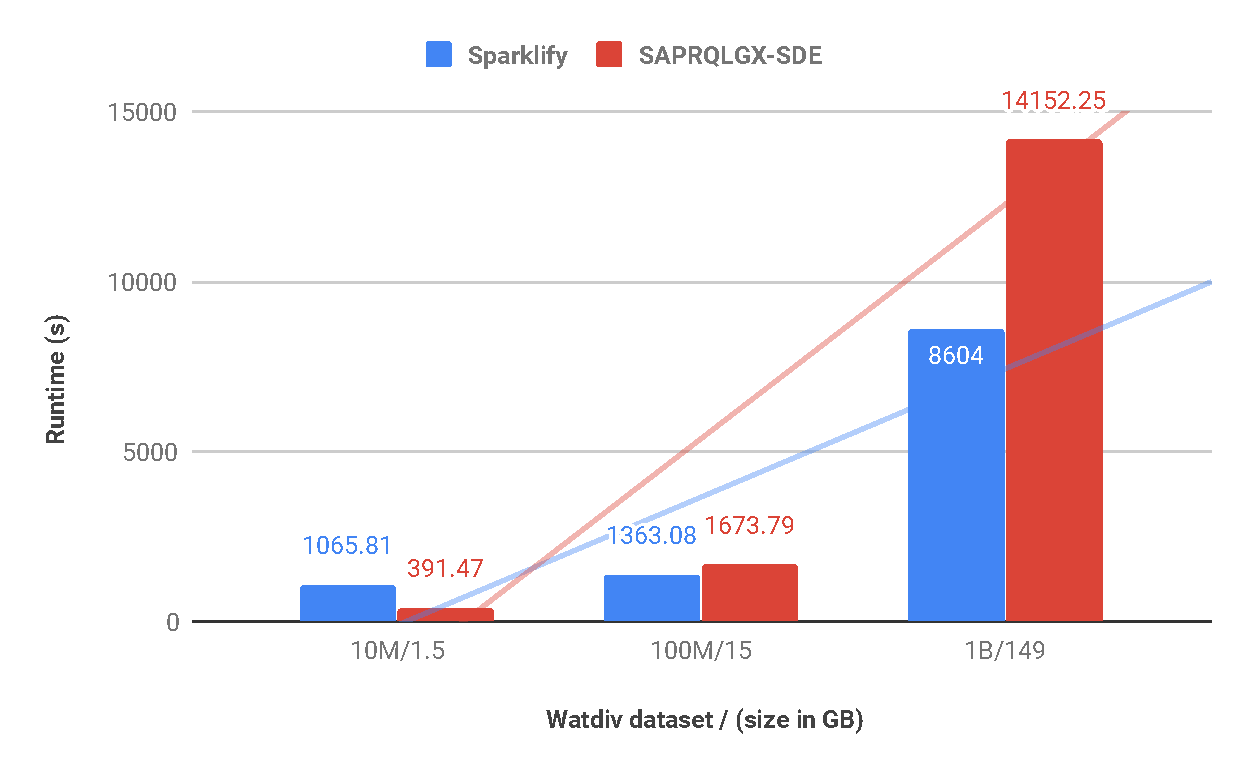
\includegraphics[width=1.0\columnwidth]{images/sizeup-scalability.pdf}
    \caption{Sizeup analysis (on Watdiv dataset).}
    \label{fig:sizeup-scalability}
\end{figure}

\defn{Size-up scalability analysis}
To measure the performance of the data scalability (e.g. size-up) of both approaches, we run experiments on three different sizes of \textit{Watdiv} (see \autoref{fig:sizeup-scalability}).
We keep the number of nodes constant i.e 6 worker nodes and grow the size of the datasets to measure whether both approaches can deal with larger datasets.
We see that the execution time for Sparklify grows linearly compared with SPARQLGX-SDE, which keeps staying as near-linear when the size of the datasets increases. 
The results presented show scalability of Sparklify in context of the sizeup, which addresses the question \ref{item:Q2}.

\defn{Node scalability analysis}
To measure the node scalability of Sparklify, we vary the number of worker nodes.
We vary them from 1, 3 to 6 worker nodes.
\autoref{fig:node-scalability} depict the speedup performance of both approaches run on \textit{Watdiv-100M} datasaet when the number of worker nodes varies.
We can see that as the number of nodes increases, the runtime cost for the Sparklify decrease linearly.
The execution time for Sparklify decreases about 0.6 times (from 2547.26 seconds down to 1588.4 seconds) as worker nodes increase from one to three nodes.
We see that the speedup stays constant when more worker nodes are added since the size of the data is not that large and the network overhead increases a little the runtime when it runs over six worker nodes.
This imply that our approach is efficient up to three worker nodes for the \textit{Watdiv-100M} (15GB) dataset.
In another hand, SPARQLGX-SDE takes longer to evaluate the queries when running on one worker node but it improves when the number of worker nodes increases.
%... \fixme{Gezim: finish this when the results are out.}

Result presented here shows that Sparklify can achieve linear scalability in the performance, which addresses \ref{item:Q3}.

\begin{figure}
  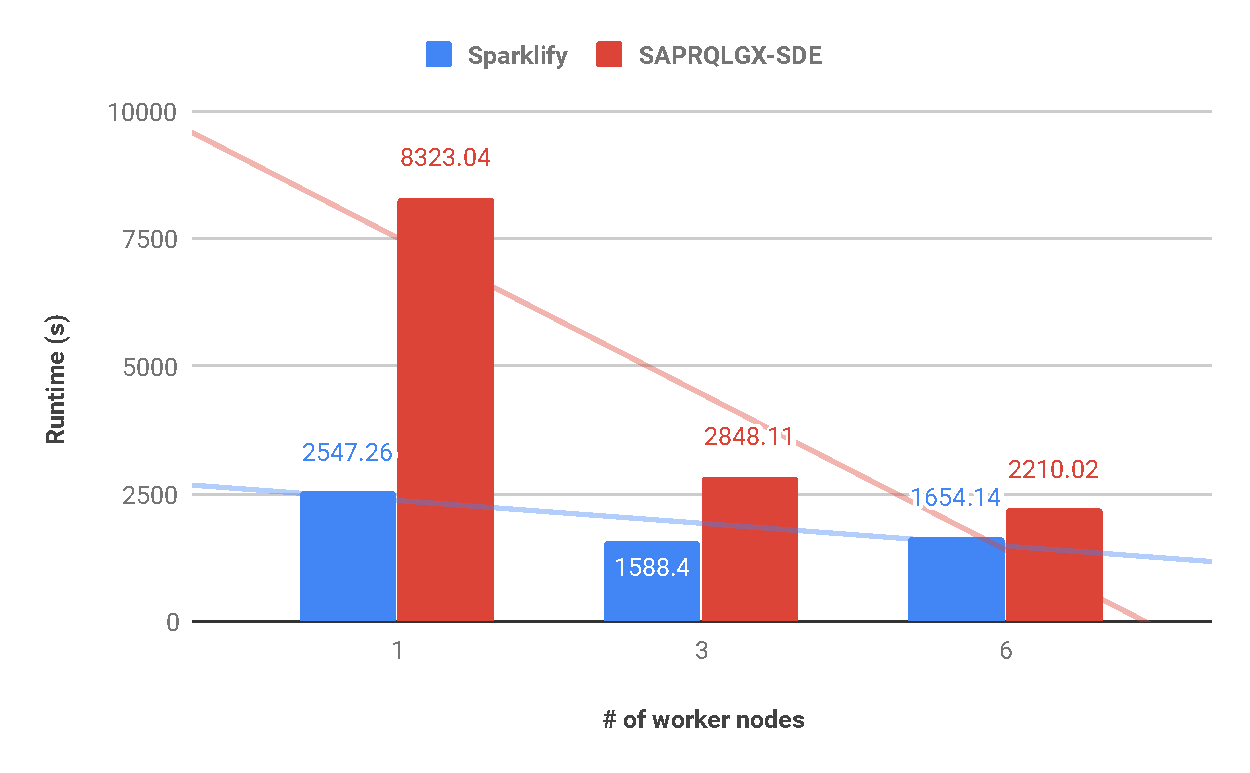
\includegraphics[width=1.0\columnwidth]{images/node-scalability.pdf}
    \caption{Node scalability (on Watdiv-100M).}
    \label{fig:node-scalability}
\end{figure}

\defn{Correctness of the result set}
In order to assess the correctness of the result set, we computed the count of the result set for the given queries and compare it within both approaches.
We conclude that both approaches return exactly the same result set which implies the correctness of the results.


\defn{Overall analysis by SPARQL queries}
Here we analyze Watdiv queries run on \textit{Watdiv-100M} dataset in a cluster mode on both approaches.
%\fixme{Gezim: Complete this part and analyze the queries which take longer for SDE on large datasets and those with takes longer for Sparklify on medium datasets.}

\begin{figure}
  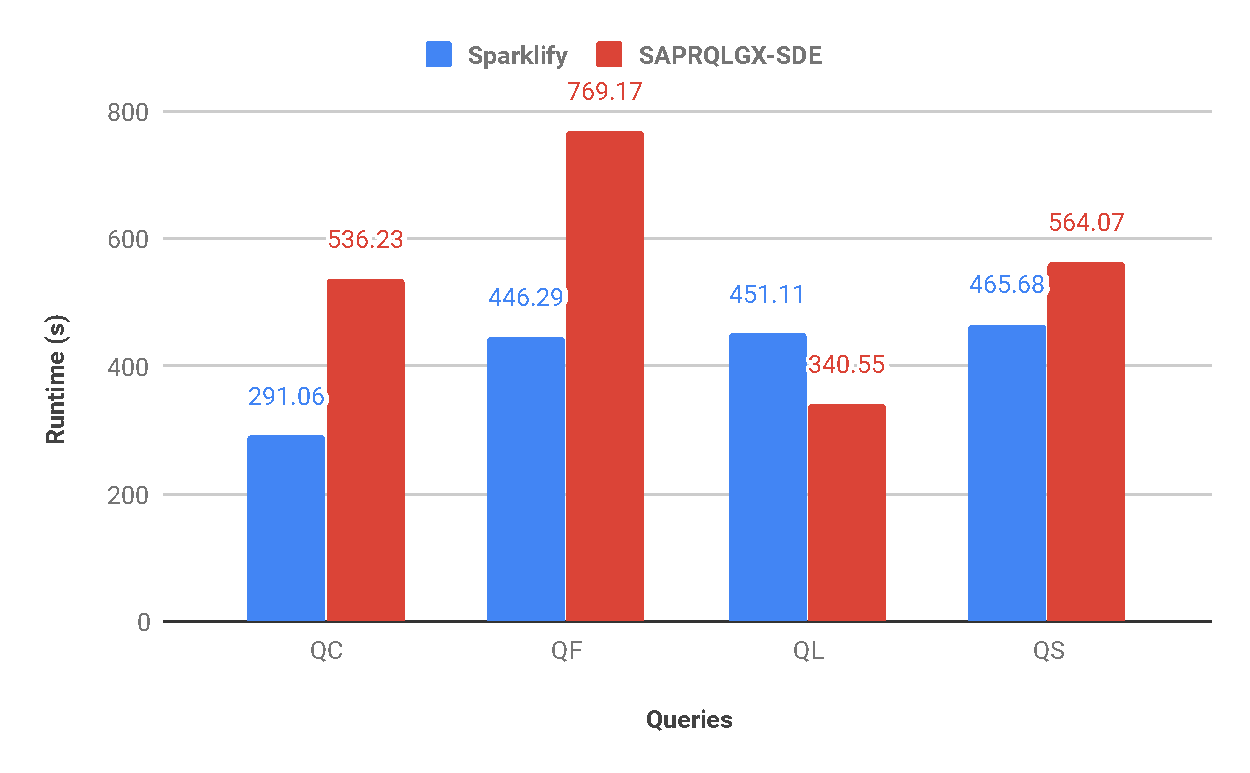
\includegraphics[width=1.0\columnwidth]{images/overall-analysis.pdf}
    \caption{Overall analysis of queries on Watdiv-100M dataset (cluser mode).}
    \label{fig:overall-analysis}
\end{figure}

%\strut\\
%\textcolor{orange}{
%    \noindent
%    Here are some ideas of discussion about the results:
%    \begin{itemize}
%        \item SDE seems not to be less performance as the number of TPs involved i the query increase. This might be due to the fact that SDE has to read the whole triple file each time.
%    \end{itemize}
%}

According to \autoref{fig:overall-analysis}, SPARQLGX-SDE performance decreases as the number of triple patterns involved in the query increase. %As it is depicted in the \autoref{fig:overall-analysis}, SPARQLGX-SDE seems to be less performance as the number of triple patterns involved in the query increase. 
This might be due to the fact that SPARQLGX-SDE has to read the whole triple file each time.
In contrast to SPARQLGX-SDE, Sparklify seems to perform well when there are more triple pattern involved (see queries \textit{QC}, \textit{QF} and \textit{QS} in the \autoref{fig:overall-analysis}) but slightly worst when there are linear queries (see \textit{QL}) evaluated. 
This may be due to the reason that Sparqlify typically rewrites a SPARQL query into a single SQL query, thus maximizing the opportunities given to the Spark SQL optimizer. Conversely, SPARQLGX-SDE constructs the workflow by chaining Scala API calls, which may restrict the possibilities e.g. in regard to join ordering.
Based on our findings and the evaluation study carried out in this paper, we show that Sparklify is scalable and the execution time ends in a reasonable time given the size of the dataset.

\section{Use Cases} 
\label{sec:use_cases}
%\fixme{Gezim: Complete this section.}

Sparklify, as a default query engine for SANSA has been used in different major use cases. 
Below, we list some of them that we are aware of using Sparklify:

\defn{Blockchain -- Alethio Use Case} Alethio\furl{https://aleth.io/} try to present the big picture of the whole Ethereum ecosystem.
It is a powerful blockchain data, analytics, and visualisation platform.
It contains more than 18 Billion triples datasets ``rdfized'' using the structure of the Ethereum ontology\furl{https://github.com/ConsenSys/EthOn}.
They are taking advantage of the SANSA stack by querying this amount of data at scale e.g. analyzing the Hubs \& Authorities in the Ethereum Transaction Network\furl{https://bit.ly/2YX7CXG} and other analytics.

\defn{SPECIAL -- A Semantic Transparency and Compliance Use Case}
SPECIAL\furl{https://www.specialprivacy.eu} is a Scalable Policy-aware Linked Data platform for privacy, transparency, and compliance.
Within the project, they introduce SPIRIT -- a transparency and compliance checking implementation of the SANSA stack.
SPECIAL uses SANSA engine in order to analyze the log information concerning personal data processing and sharing that as an output from line of business applications on a continuous basis, and to present the information to the user via the SPIRIT dashboard.
The SPIRIT transaction log processing allows users to: (1) define the set of policies rules, (2) initialize the query engine with the log and schema/ontology data, here is where Sparklify is used in specific, (3) create a reasoner set reasoning profile, and (4) apply these rules to the given query in order be compliant with the policy rules.

\defn{SLIPO -- Categorizing Areas of Interests (AOI) Use Case} SLIPO\furl{http://slipo.eu/} take advantage of the Semantic Web Technologies for the scalable and efficient integration of Big Point of Interest (POI) datasets.
In particular, the project focuses on designing efficient pipelines dealing with large semantic datasets of POIs: a wide range of features are available inter alia fusion \& cleaning distinct datasets or detection of future ``hot'' AOIs where businesses should be created.
In this project, Sparklify is used through the SANSA query layer to refine, filter and select the relevant POIs which are needed by the pipelines.

%\defn{QROWD -- Something}
%QROWD\furl{http://qrowd-project.eu/} is a cross-sectorial project which offers local government and transportation businesses innovative solutions to improve mobility, reduce traffic congestion and make navigation safer and more efficient. 
%In order to achieve this, QROWD integrate different sources of data by leveraging the value of Big Data processing engine and semantic web technologies.
%One of the challenges to be tackled in QROWD is the disambiguation while crawling the data. 
%\fixme{Gezim-to-Claus: I think you know it better to explain it.}






\section{Related Work}
\label{sec:related_work}

As our main focus is on the area of distributed computing, we omit the centralized systems e.g. RDF-3X~\cite{Neumann2008RRE} or Virtuoso~\cite{Erling2010} (see~\cite{faye2012survey} for a survey) and we review the distributed ones only (see~\cite{kaoudi2015rdf} for a recent survey).
Further, this set of tools is divided into: \textit{MapReduce-based} systems and \textit{In-Memory} systems e.g. on top of Apache Spark.

\textit{MapReduce systems} -- SHARD~\cite{Rohloff2010} is one approach which groups RDF data into a dedicated partition so-called semantic-based partition. 
It groups these RDF data by subject and implements a query engine which iterates through each of the clauses used on the query and performs a query processing.
A MapReduce job is created while scanning each of the triple patterns and generates a single plan for each of the triple pattern which leads to a larger query plan, therefore, it contains too many Map and Reduces jobs.
PigSPARQL~\cite{Schatzle2011PMS} is yet another approach which uses Hadoop based implementation of vertical partitioning for data representation. 
It translated the SPARQL queries into Pig\furl{https://pig.apache.org/} LATIN queries and uses Pig as an intermediate engine.
Another approach which is based on the MapReduce is Sempala~\cite{Schatzle2014Sempala} -- as SPARQL-to-SQL approach on top of Hadoop.
It uses Impala\furl{https://impala.apache.org/} as a distributed SQL processing engine.
Sempala uses a so-called unified vertical partitioning (single property table) in order to boost the star-shaped queries by excluding the joins.
Hence, its limitation is that it is designed only to that particular shape of the queries.
RYA~\cite{Punnoose2012Rya} is a Hadoop based scalable RDF store that uses Accumulo\furl{https://accumulo.apache.org} as a distributed key-value store for indexing the RDF triples.
RYA indexes triples into three tables and replicate them across the cluster for leveraging the indexes over all the possible records.
It has the mechanism of performing join reorder, but it lacks of the in-memory computation, which makes it not comparable with other systems.
While the MapReduce paradigm has been realized for disk-based as well as in-memory processing, the concept is not concerned with controlling aspects of general distributed workflows, such as which intermediate results to cache. As a consequence, high level frameworks were devised which may use MapReduce as a building block.%The drawback of using the MapReduce paradigm is the usage of the disk-based processing, therefore, the new solution came out.
Apache Spark is one of them~\cite{zaharia2012resilient}.
Below, we will list some of the approaches which make use of the Apache Spark (in-memory computation) framework. 

\textit{In-Memory systems} --
SPARQLGX~\cite{sparqlgx-iswc-2016} and S2RDF~\cite{Schatzle:2016:SRQ:2977797.2977806} approaches are considered the most recent distributed SPARQL evaluators over large-scale RDF datasets.
SPARQLGX is a scalable query engine which is capable of evaluating efficiently the SPARQL queries over distributed RDF datasets~\cite{graux2018multi}.
It provides a mechanism for translating SPARQL queries into Spark executable code for better leveraging the advantage of the Spark framework.
It uses a simplified VP approach, where each predicate is assigned with a specific parquet file. 
As an addition, it is able to assign RDF statistics for further query optimization while also providing the possibility of directly query files on the HDFS using SDE.
S2RDF is similar to SPARQLGX, but instead of dealing with direct Spark code (aka RDDs), it translates SPARQL queries into SQL ones run by Spark-SQL. 
It introduces a data partitioning strategy that extends VP with additional statistics, containing pre-computed semi-joins for query optimization.


\section{Conclusions and Future Work}
\label{sec:conclusion}
Querying RDF data becomes challenging when the size of the data increases.
%Existing systems mostly contain a very moderately information of the data while transforming them to a dedicated storage model (e.g. vertical partitioning).
%contain a very moderately information of the data
Existing Spark-based SPARQL systems mostly
do not retain all RDF term information consistently while transforming them to a dedicated storage model such as using vertical partitioning.
Often, this process is both data and computing intensive and raises the need for a scalable, efficient and comprehensive query engine which can handle large scale RDF datasets.

In this paper, we propose \emph{Sparklify}: a scalable software component for efficient evaluation of SPARQL queries over distributed RDF datasets. 
It uses Sparqify as a SPARQL-to-SQL rewriter for translating SPARQL queries into Spark executable code.
By doing so, it leverages the advantages of the Spark framework.
SANSA features methods to execute SPARQL queries directly as part of Spark workflows instead of writing the code corresponding to those queries (sorting, filtering, etc.).
It also provides a command-line interface and a W3C standard compliant SPARQL endpoint for externally querying data that has been loaded using the SANSA framework.
We have shown empirically that our approach can scale horizontally and perform well w.r.t to the state-of-the-art approaches.

With this work, we showed that the application of OBDA tooling to Big Data frameworks achieves promising results in terms of scalability. 
We present a working prototype implementation that can serve as a baseline for further research. 
Our next steps include evaluating other tools, such as Ontop~\cite{Calvanese2017OntopAS}, and analyze how their performance in the Big Data setting can be improved further. 
For example, we intend to investigate how OBDA tools can be combined with dictionary encoding of RDF terms as integers and evaluate the effects.

%Although we have achieved %reasonable results in %terms of scalability, we %further plan to cover more %SPARQL fragments.

%\section*{Acknowledgment}
%This work was partly supported by the EU Horizon2020 projects BigDataOcean (GA no.~732310), Boost4.0 (GA no.~780732), SLIPO (GA no.~731581) and QROWD (GA no.~723088); and by the ADAPT Centre for Digital Content Technology funded under the SFI Research Centres Programme (Grant 13/RC/2106) and co-funded under the European Regional Development Fund.

%\bibliographystyle{abbrv}
%\bibliography{references}

%\clearpage 

%{\huge Pages: \the\numexpr\value{page}-1\relax{} (Limit: 16)}

%\end{document}

